\documentclass{beamer}
\usetheme{Warsaw}
\usepackage[utf8]{inputenc}
\usepackage[ngerman]{babel}
\usepackage{listings}
\usepackage{color}

\lstdefinelanguage{JavaScript}{
  keywords={typeof, new, true, false, catch, function, return, null, catch, switch, var, if, in, while, do, else, case, break},
  keywordstyle=\color{blue}\bfseries,
  ndkeywords={class, export, boolean, throw, implements, import, this},
  ndkeywordstyle=\color{darkgray}\bfseries,
  identifierstyle=\color{black},
  sensitive=false,
  comment=[l]{//},
  morecomment=[s]{/*}{*/},
  commentstyle=\color{purple}\ttfamily,
  stringstyle=\color{red}\ttfamily,
  morestring=[b]',
  morestring=[b]"
}

\lstset{
   language=JavaScript,
   backgroundcolor=\color{lightgray},
   extendedchars=true,
   basicstyle=\footnotesize\ttfamily,
   showstringspaces=false,
   showspaces=false,
   numbers=left,
   numberstyle=\footnotesize,
   numbersep=9pt,
   tabsize=2,
   breaklines=true,
   showtabs=false,
   captionpos=b
}

\title{Monitoringsystem einer Ambient Assisted Living-Anwendung mit Hilfe der eXist Datenbank}
\author{Adam Kucera, Andre Krause, Robert Riedel}
\date{\today}

\begin{document}
\maketitle
\begin{frame}
	\frametitle{Inhalt}
	\tableofcontents[%
% 		currentsection, % causes all sections but the current to be shown in a semi-transparent way.
% 		currentsubsection, % causes all subsections but the current subsection in the current section to ...
% 		hideallsubsections, % causes all subsections to be hidden.
 		hideothersubsections, % causes the subsections of sections other than the current one to be hidden.
% 		part=, % part number causes the table of contents of part part number to be shown
%		pausesections, % causes a \pause command to be issued before each section. This is useful if you
% 		pausesubsections, %  causes a \pause command to be issued before each subsection.
% 		sections={ overlay specification },
	]
\end{frame}

\section{Problemstellung}
\begin{frame}
\frametitle{Problemstellung}
\begin{itemize}
	\item Anteil älterer Menschen nimmt zu
	\item Betreuung in eigenen vier Wänden schwierig
	\item Möglichkeit muss gefunden werden, dies zu ermöglichen
	\item Einsatz technischer Hilfsmittel
	%\item Ambient Assisted Living (AAL) = 
\end{itemize}
\begin{Definition}
Ambient Assisted Living (AAL) ist die Vernetzung des Wohnraums an sich und mit externen Dienstleistern zur alltäglichen Unterstützung und Überwachung.
\end{Definition}
\end{frame}

\section{Aufgabenstellung}
\begin{frame}
\frametitle{Aufgabenstellung}
\begin{itemize}
	\item Überwachung der Vitalwerte durch Sensoren
	\item In Wänden oder am Handgelenk
	\item Senden Werte an zentrale Stelle
	\item In Datenbank abgespeichert
	\item An Monitoring System weitergeleitet
\end{itemize}
\end{frame}

\begin{frame}
\frametitle{Aufgabenstellung}
\begin{itemize}
	\item Erstellen einer Server-Client Anwendung mit Hilfe von XML-Technologien
	\item eXist als Datenbank
	\item Webclient zur Anzeige der Vitalwerte
	\item Reporterstellung
\end{itemize}
\end{frame}

\section{Entwurf}
\begin{frame}
\frametitle{Use-Cases}
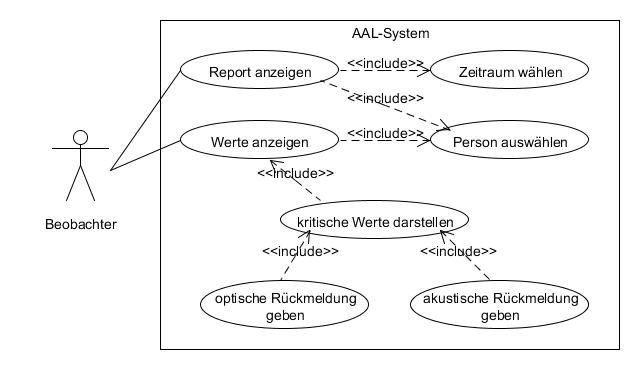
\includegraphics[scale=0.5]{images/AAL-Use-Case-Diagramm.jpg} 
\end{frame}

\begin{frame}
\frametitle{Technologien}
\begin{itemize}
	\item eXist
	\item HTML5+Javascript
	\item Node.JS
	\item XML
	\item XQuery
	\item XSLT - XSL-FO - PDF
	\item REST
	\item Websockets
\end{itemize}
\end{frame}

\begin{frame}
\frametitle{System-Architektur}
\begin{figure}[H]
\begin{center}
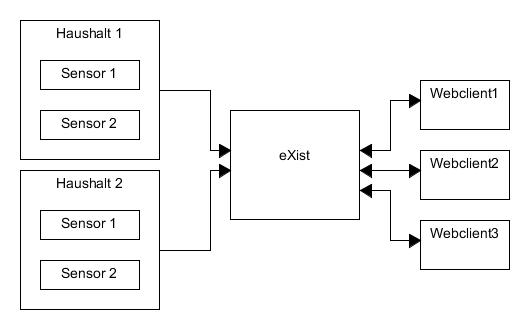
\includegraphics[scale=0.5]{images/sa1.jpg} 
\end{center}
\end{figure}
\end{frame}

\begin{frame}
\frametitle{System-Architektur}
\begin{figure}[H]
\begin{center}
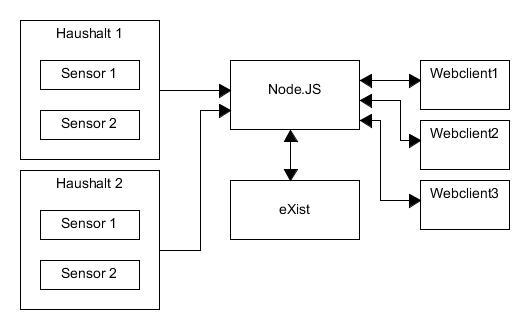
\includegraphics[scale=0.5]{images/sa2.jpg} 
\end{center}
\end{figure}
\end{frame}


\begin{frame}[fragile]
\frametitle{Kommunikation}
\begin{itemize}
	\item XML für Sensorwerte
\end{itemize}
\begin{lstlisting}
<sensorData>
    <personId>1</personId>
    <roomId>1</roomId>
    <timestamp>
		         <time>19:42 PM</time><date>2015-05-13</date>
		         </timestamp>
    <sensor>
		         <type>Blutdruck</type>
		         <value>123</value>
    </sensor>
</sensorData>
\end{lstlisting}
\end{frame}

\section{Implementierung}

\begin{frame}[fragile]
\frametitle{Implementierung}
\begin{itemize}
	\item Websocket
\end{itemize}
\begin{lstlisting}
var socketio = require('socket.io');

socket.on("disconnect", function(){
            console.log("Client mit id: " + socket.id + " disconnected!");
            hmap.forEach(function (value, key) {
                if(key==socket.id){
                    hmap.remove(key);
                }
            });
        });
        
receiver.emit("receiveVitalWert", xml);
\end{lstlisting}
\end{frame}

\begin{frame}[fragile]
\begin{itemize}
	\item Websocket - Webclient
\end{itemize}
\begin{lstlisting}
function getPersonData() {
    person = document.getElementById("personID");
    personID = person.value;
    setTextById("personErrorField","");
    reportButton = document.getElementById("getReportButton");
    if(personID==""){
        reportButton.disabled="disabled";
        setTextById("personErrorField","personID darf nicht leer sein");
    } else{
        reportButton.disabled="";
        socket.emit("setPersonId", personID);
        console.log("sent request for personId: #"+personID+"#");    
    }
}
\end{lstlisting}
\end{frame}

\begin{frame}[fragile]
\begin{lstlisting}
socket.on("receiveVitalWert", function (xml) {
    dom = domify(xml);
    person = dom.getElementsByTagName("personId")[0].firstChild.nodeValue;
    setTextById('person', person);
    room = dom.getElementsByTagName("roomId")[0].firstChild.nodeValue;
    setTextById('room', room);
    type = dom.getElementsByTagName("type")[0].firstChild.nodeValue;
    ...
    date = dom.getElementsByTagName("date")[0].firstChild.nodeValue;
    setTextById(type + 'Date', date);
    if (status == 'normal') {
        setNormalClass(type);
    } else {
        setCriticalClass(type);
    }
});
\end{lstlisting}
\end{frame}

\begin{frame}[fragile]
\begin{itemize}
	\item  Ton für kritische werte
\end{itemize}
\begin{lstlisting}
<audio id="HerzfrequenzCritSound" loop="loop">
    <source src="sirene-airRaid.mp3" type="audio/mpeg"/>
    Your browser does not support the audio element.
</audio>
\end{lstlisting}
\begin{lstlisting}
function activateSound(id) {
    console.log("play sound of: #" + id + '#');
    elementToChange = document.getElementById(id);
    if(playSound){
    elementToChange.play();
    }else{
        deActivateSound(id);
    }
}
\end{lstlisting}
\end{frame}

\begin{frame}[fragile]
\begin{itemize}
	\item REST-Service
\end{itemize}
\begin{lstlisting}
function route(handle, pathname, response, request) {
    if(typeof handle[pathname] === 'function'){
        handle[pathname](response, request);
    } else {
        console.log("No request handler found for " + pathname);
        response.writeHead(404, {"Content-Type": "text/plain"});
        response.write("404 Not found");
        response.end();
    }
}

handle["/postVitalwert"] = vitalWerteHandler.postVitalwert;
\end{lstlisting}

\end{frame}

\begin{frame}[fragile]
\begin{lstlisting}
client.post("http://localhost:8080/exist/restxq/postSensorData", args, function(data,response) {
                var string = data.message;
            });
\end{lstlisting}
\end{frame}



\begin{frame}[fragile]
\begin{lstlisting}
let $table-fo := transform:transform($tableBody,doc("/db/apps/aal-server/test-xsl.xsl"),())
let $fo := <fo:root xmlns:fo="http://www.w3.org/1999/XSL/Format">
                <fo:layout-master-set>
                    <fo:simple-page-master master-name="my-page">
                        <fo:region-body margin="1in"/>
                    </fo:simple-page-master>
                </fo:layout-master-set>
   
\end{lstlisting}
\end{frame}   
                
\begin{frame}[fragile]
\begin{lstlisting}                
                
                <fo:page-sequence master-reference="my-page">
                    <fo:flow flow-name="xsl-region-body">
                        <fo:block>
                            {$table-fo}
                        </fo:block>
                    </fo:flow>
                </fo:page-sequence>
          </fo:root>
let $pdf := xslfo:render($fo, "application/pdf", ())
\end{lstlisting}
\end{frame}

\begin{frame}
\begin{itemize}
\item Vorführung
\end{itemize}
\end{frame}

\section{Probleme}
\begin{frame}
\frametitle{Probleme}
\begin{itemize}
	\item XQWebsocketModule nicht mehr für aktuelle Version
	\item Nicht alle XQuery-Funktionen implementiert
\end{itemize}
\end{frame}

\section{Fazit}
\begin{frame}
\frametitle{Fazit}
\begin{itemize}
	\item Use-Cases umgesetzt
	\item GUI durch Diagramm erweitern
	\item neue Reportmöglichkeiten
	\item Login-Funktion
	\item Echtzeittests
\end{itemize}
\end{frame}

\begin{frame}
\begin{center}
\Huge Fragen?
\end{center}

\end{frame}

\end{document}